\documentclass{report}
% --- Core ---
\usepackage[utf8]{inputenc}
\usepackage[T1]{fontenc}
\usepackage[margin=2.5cm]{geometry}
\usepackage{enumitem}

% --- Math & Symbols ---
\usepackage{amsmath, amssymb, amsfonts, amsthm}
\usepackage{cancel}

% --- UI & Layout ---
\usepackage{parskip} % Spasi antar paragraf, tanpa indentasi
\usepackage{float}
\usepackage{graphicx}
\usepackage{caption}
\usepackage{subcaption} % Untuk sub-figures
\usepackage{booktabs}   % Tabel cantik ( \toprule, \midrule, \bottomrule )
\usepackage{array}
\usepackage{lipsum}

% --- Colors & Links ---
\usepackage[dvipsnames]{xcolor}
\usepackage{hyperref}

% --- Code Snippets (Listings) ---
\usepackage{listings}
\definecolor{codegreen}{rgb}{0,0.6,0}
\definecolor{codegray}{rgb}{0.5,0.5,0.5}
\definecolor{codepurple}{rgb}{0.58,0,0.82}
\definecolor{backcolour}{rgb}{0.95,0.95,0.92}

\lstset{
    backgroundcolor=\color{backcolour},   
    commentstyle=\color{codegreen},
    keywordstyle=\color{magenta},
    numberstyle=\tiny\color{codegray},
    stringstyle=\color{codepurple},
    basicstyle=\ttfamily\small,
    breakatwhitespace=false,         
    breaklines=true,                 
    captionpos=b,                    
    keepspaces=true,                 
    numbers=left,                    
    numbersep=5pt,                  
    showspaces=false,                
    showstringspaces=false,
    showtabs=false,                  
    tabsize=2
}

% --- Diagrams (TikZ) ---
\usepackage{tikz}
\usepackage{tikz-network}
\usetikzlibrary{trees, graphs, arrows.meta, shapes.geometric, positioning}

% --- Boxes (tcolorbox) ---
\usepackage[breakable]{tcolorbox}
\tcbuselibrary{theorems}

\newtcbtheorem[number within=chapter]{definisi}{Definisi}%
{breakable, colback=green!5,colframe=green!35!black,fonttitle=\bfseries}{def}

\newtcbtheorem[number within=chapter]{teorema}{Teorema}%
{breakable, colback=blue!5,colframe=blue!35!black,fonttitle=\bfseries}{th}

\newtcbtheorem[number within=chapter]{contoh}{Contoh}%
{breakable, colback=red!5,colframe=red!35!black,fonttitle=\bfseries}{ex}

% --- Header & Footer ---
\usepackage{fancyhdr}
\pagestyle{fancy}
\fancyhf{}
\fancyhead[L]{\small IF4031 - JagaWarga}
\fancyhead[R]{\small \leftmark}
\fancyfoot[C]{\thepage}

% --- Referencing ---
\usepackage[noabbrev, capitalize]{cleveref}
\graphicspath{{images/}}

\renewcommand{\contentsname}{Daftar Isi}
\renewcommand{\chaptername}{Bab}
\renewcommand{\figurename}{Gambar}
\renewcommand{\tablename}{Tabel}
\renewcommand{\bibname}{Daftar Pustaka} % Untuk document class report/book

\hypersetup{
    colorlinks=true,
    linkcolor=black,
    filecolor=magenta,      
    urlcolor=cyan,
    pdftitle={Tugas Besar IF4031 Arsitektur Aplikasi Terdistribusi},
}

\begin{document}

% --- Mulai Cover ---
\begin{titlepage}
    \centering
    
    % Judul Mata Kuliah
    \Large \textsf{Tugas Besar IF4031 Arsitektur Aplikasi Terdistribusi} \\
    \vspace{1.5cm}

    % Judul Project
    \huge \textbf{JagaWarga: \\ Aplikasi Pelaporan Warga Dengan Arsitektur Terdistribusi} \\
    \vspace{1.5cm}

    % Foto cover
    \includegraphics[width=0.4\textwidth]{cover.jpg} \\ 
    \vspace{1.5cm}

    % Penulis
    \large \textit{Disusun oleh: Kelompok anomali\_nangor} \\
    \vspace{0.5cm}
    
    \begin{tabular}{r l}
        Rhio Bimo Prakoso Sugiyanto & 13523123 \\
        Frederiko Eldad Mugiyono & 13523147 \\
        Naufarrel Zhafif Abhista & 13523149
    \end{tabular}

    \vfill

    \large
    Program Studi Teknik Informatika \\
    Sekolah Teknik Elektro dan Informatika \\
    Institut Teknologi Bandung \\
    2025
\end{titlepage}

\pagenumbering{roman}
\tableofcontents
\newpage

\pagenumbering{arabic}
\setcounter{page}{1}

\chapter{Pembagian Tugas}

\section{Tim Pelaksana}

Implementasi JagaWarga PoC dilakukan oleh tiga anggota tim dengan pembagian tanggung jawab sebagai berikut:

\begin{table}[H]
\centering
\caption{Pembagian Tugas dan Tanggung Jawab}
\label{tab:pembagian_tugas}
\begin{tabular}{|p{4cm}|p{2.5cm}|p{7.5cm}|}
\hline
\textbf{Nama} & \textbf{NIM} & \textbf{Tanggung Jawab Utama} \\
\hline
Rhio Bimo Prakoso Sugiyanto & 13523123 & 
\begin{itemize}[nosep]
  \item Identity Service (JWT validation mock)
  \item Anonymizer Service (PII scrubbing pipeline)
  \item NATS event publisher
  \item Integration testing scripts
\end{itemize} \\
\hline
Frederiko Eldad Mugiyono & 13523147 & 
\begin{itemize}[nosep]
  \item CockroachDB schema design \& encryption
  \item NATS JetStream configuration
  \item Traefik TLS setup
  \item Prometheus + Grafana observability
  \item Docker Compose orchestration
\end{itemize} \\
\hline
Naufarrel Zhafif Abhista & 13523149 & 
\begin{itemize}[nosep]
  \item Report Service (Phoenix/Ecto)
  \item Escalation Worker (GenServer)
  \item NATS event publisher integration
  \item Database optimization
  \item Prometheus metrics exporter
\end{itemize} \\
\hline
\end{tabular}
\end{table}

\section{Deliverables per Tim}

\subsection{Tim Infrastructure \& Security (Frederiko Eldad Mugiyono)}
\begin{itemize}
  \item Database schema dengan encryption-at-rest di CockroachDB
  \item Konfigurasi NATS JetStream streams
  \item Self-signed TLS certificates
  \item Prometheus scrape configuration
  \item Grafana dashboard dengan 4 panel monitoring
  \item Seed data script (100 fake citizens, 5 authorities)
  \item Docker Compose dengan health checks lengkap
\end{itemize}

\subsection{Tim Backend Services (Naufarrel Zhafif Abhista)}
\begin{itemize}
  \item Phoenix Report Service dengan CRUD operations
  \item Escalation Worker (GenServer + Quantum scheduler)
  \item API endpoints: \texttt{POST /reports}, \texttt{GET /reports?department=X}
  \item Background job untuk auto-escalation stale reports (timeout 30s)
  \item Health check endpoint: \texttt{GET /health}
  \item Metrics endpoint: \texttt{GET /metrics} (format Prometheus)
  \item Database connection pooling \& query optimization
\end{itemize}

\subsection{Tim Edge Services (Rhio Bimo Prakoso Sugiyanto)}
\begin{itemize}
  \item Identity Service dengan JWT validation mock
  \item Anonymizer Service dengan pipeline PII scrubbing
  \item NATS event publisher untuk report.created events
  \item Dockerfiles untuk Bun services
  \item Request/response logging \& error handling
  \item Load test script (submit 100 anonymous reports)
  \item API documentation \& usage examples
\end{itemize}

\chapter{Pendahuluan}

\section{Latar Belakang}
Pertumbuhan populasi perkotaan yang pesat membawa tantangan besar dalam pengelolaan infrastruktur, keamanan, dan kebersihan lingkungan. Kota dengan estimasi penduduk sebanyak 2,5 juta jiwa memerlukan mekanisme komunikasi yang efisien antara warga dan pemerintah. Sistem pelaporan masalah konvensional seringkali mengalami hambatan dalam hal kecepatan respon, transparansi status, dan ketepatan distribusi laporan ke pihak yang berwenang.

Aplikasi JagaWarga dirancang sebagai platform pelaporan terintegrasi yang memungkinkan warga melaporkan permasalahan mulai dari kriminalitas hingga perawatan fasilitas umum. Namun, mengelola basis pengguna sebesar 2,5 juta dengan volume data multimedia yang masif dan kebutuhan akan fitur privasi (anonimitas) menimbulkan kompleksitas teknis yang signifikan. Arsitektur monolitik dianggap tidak lagi memadai untuk menangani kebutuhan ini karena keterbatasan dalam skalabilitas horizontal dan risiko \textit{single point of failure}.


\section{Identifikasi Masalah}
Berdasarkan latar belakang tersebut, permasalahan utama yang diidentifikasi dalam pengembangan sistem ini adalah:
\begin{enumerate}
    \item \textbf{Skalabilitas Sistem:} Bagaimana menangani lonjakan beban laporan yang mendadak dari jutaan pengguna tanpa menurunkan performa aplikasi secara keseluruhan.
    \item \textbf{Isolasi Data dan Keamanan:} Bagaimana memastikan laporan hanya dapat diakses oleh instansi yang berwenang (misal: Dinas Kebersihan tidak dapat melihat laporan kriminalitas) serta menjamin anonimitas bagi \textit{whistleblower}.
    \item \textbf{Reliabilitas dan Ketersediaan:} Bagaimana merancang sistem yang tetap berfungsi meskipun salah satu komponen atau layanan mengalami kegagalan.
    \item \textbf{Eskalasi dan Pemantauan:} Bagaimana mengotomatisasi proses eskalasi laporan yang tidak tertangani serta memungkinkan otoritas tertinggi memantau kinerja jajaran di bawahnya secara \textit{real-time}.
\end{enumerate}

\section{Tujuan Tugas Besar}
Tujuan dari perancangan dan implementasi \textit{Proof-of-Concept} (PoC) pada tugas besar ini adalah:
\begin{enumerate}
    \item Merancang arsitektur aplikasi terdistribusi yang mampu memenuhi aspek keamanan, keandalan, dan skalabilitas.
    \item Mengimplementasikan sistem pelaporan yang mendukung berbagai tingkat privasi (publik, privat, anonim).
    \item Menerapkan mekanisme \textit{observability} untuk memantau trafik dan performa antar komponen sistem.
    \item Membuktikan efektivitas arsitektur terdistribusi dalam menangani fungsionalitas kritis seperti eskalasi otomatis dan isolasi data.
\end{enumerate}
\chapter{Spesifikasi Kebutuhan Perangkat Lunak}

\section{Deskripsi Kebutuhan}
Sistem \textit{JagaWarga} dirancang untuk memfasilitasi pelaporan permasalahan warga di lingkungan perkotaan dengan populasi besar. Sistem ini memastikan setiap laporan diteruskan secara tepat sasaran kepada pihak berwenang terkait, menjaga privasi pelapor melalui fitur anonimitas, serta menyediakan mekanisme pemantauan kinerja bagi otoritas tertinggi. Berdasarkan kebutuhan klien, sistem ini harus diimplementasikan menggunakan arsitektur terdistribusi untuk menjamin kualitas layanan pada skala besar.

\section{Kebutuhan Fungsional Produk}
Berikut adalah daftar kebutuhan fungsional yang harus dipenuhi oleh sistem:

\begin{enumerate}[label=\textbf{FR-\arabic*}, leftmargin=1.5cm]
    \item Warga dapat melaporkan masalah dalam bentuk laporan tertulis yang dilengkapi dengan lokasi dan multimedia. Laporan dapat bersifat \textit{publik}, \textit{privat}, atau \textit{anonim} (\textit{whistleblowing}).
    \item Warga dapat mengelola laporan pribadi serta memantau status penyelesaiannya.
    \item Warga dapat melihat laporan publik lain dan memberikan \textit{upvote} sebagai bentuk dukungan.
    \item Sistem dapat mengirimkan notifikasi kepada pelapor saat terdapat kemajuan pada penyelesaian laporan.
    \item Pihak berwenang dapat memantau dan merespon masalah yang terkait dengan kewenangannya secara \textit{real-time}.
    \item Pihak berwenang dapat melakukan analisis data terkait masalah-masalah yang dilaporkan.
    \item Pihak berwenang dapat meneruskan laporan ke aplikasi atau sistem eksternal yang sudah ada.
    \item Sistem dapat mengeskalasi laporan ke pihak dengan kewenangan lebih tinggi apabila tidak berhasil ditangani dalam waktu tertentu.
    \item Kewenangan tertinggi dapat memantau kinerja bawahan dalam menanggapi masalah yang dilaporkan.
\end{enumerate}

\section{Kebutuhan Non-fungsional Produk}
Kebutuhan non-fungsional atau atribut kualitas yang wajib dipenuhi adalah sebagai berikut:

\subsection{Keamanan (\textit{Security})}
\begin{enumerate}[label=\textbf{NFR-S\arabic*}, leftmargin=1.7cm]
    \item \textbf{Pemisahan Masalah:} Pihak penerima laporan hanya dapat melihat masalah di bawah wewenangnya (isolasi data berdasarkan jenis masalah).
    \item \textbf{Anonimitas:} Pelapor dapat memberikan laporan tanpa identitas yang dapat dilacak.
    \item \textbf{Validasi Identitas:} Sistem mampu memvalidasi identitas pelapor untuk memastikan data tidak dipalsukan.
    \item \textbf{Proteksi Data Pribadi:} Sistem wajib menghilangkan seluruh data pribadi pada pembuat laporan anonim.
    \item \textbf{Keamanan Data:} Menjaga keamanan data baik saat dikirimkan (\textit{in-transit}) maupun saat disimpan (\textit{at-rest}).
\end{enumerate}

\subsection{Keandalan (\textit{Reliability})}
\begin{enumerate}[label=\textbf{NFR-R\arabic*}, leftmargin=1.7cm]
    \item \textbf{Fault Isolation:} Kegagalan pada satu \textit{instance} atau komponen tidak menyebabkan kegagalan total pada keseluruhan aplikasi.
\end{enumerate}

\subsection{Skalabilitas (\textit{Scalability})}
\begin{enumerate}[label=\textbf{NFR-SC\arabic*}, leftmargin=1.7cm]
    \item \textbf{Lonjakan Beban:} Mampu menangani lonjakan beban pengguna yang mendadak dan tidak terduga.
    \item \textbf{Efisiensi Sumber Daya:} Mampu mengurangi penggunaan sumber daya ketika beban sedang rendah.
\end{enumerate}

\subsection{Kinerja (\textit{Performance})}
\begin{enumerate}[label=\textbf{NFR-P\arabic*}, leftmargin=1.7cm]
    \item \textbf{Response Time:} Memberikan waktu respon sistem yang memuaskan bagi pengguna.
\end{enumerate}

\subsection{Observabilitas (\textit{Observability})}
\begin{enumerate}[label=\textbf{NFR-O\arabic*}, leftmargin=1.7cm]
    \item \textbf{Monitoring Sistem:} Memungkinkan tim infrastruktur memantau kinerja keseluruhan dan melacak lalu lintas antar komponen.
    \item \textbf{Monitoring Keamanan:} Memungkinkan tim keamanan memantau lalu lintas sistem dengan tetap menjaga privasi pengguna.
\end{enumerate}
\chapter{Perancangan Sistem}

\section{Deskripsi Umum Sistem}
Sistem \textit{JagaWarga} dirancang dengan pendekatan arsitektur \textit{microservices} untuk menangani kompleksitas pelaporan warga pada kota berpenduduk 2,5 juta jiwa. Berbeda dengan pendekatan monolitik, sistem ini memecah fungsionalitas utama menjadi layanan-layanan kecil yang independen dan saling berkomunikasi melalui protokol jaringan. Hal ini dilakukan untuk menjamin bahwa lonjakan beban pada satu fitur (misalnya lonjakan pelaporan saat banjir) tidak melumpuhkan fungsi lain seperti analisis data oleh pihak berwenang.



Secara garis besar, sistem terdiri dari beberapa komponen utama yang bekerja secara terintegrasi:
\begin{enumerate}
    \item \textbf{Edge Layer (Gateway):} Bertindak sebagai pintu masuk tunggal bagi seluruh permintaan dari aplikasi warga dan portal dinas. Di lapisan ini dilakukan \textit{rate limiting} dan \textit{load balancing} untuk menjaga stabilitas sistem dari beban mendadak.
    \item \textbf{Core Services:} Terdiri dari kumpulan layanan yang menangani logika bisnis inti. 
    \begin{itemize}
        \item \textit{Identity Service} mengelola validasi pengguna.
        \item \textit{Report Service} mengelola siklus hidup laporan.
        \item \textit{Anonymizer Proxy} memastikan data pelapor anonim dibersihkan sebelum disimpan di basis data laporan.
    \end{itemize}
    \item \textbf{Asynchronous Processing:} Menggunakan \textit{Message Broker} sebagai jembatan komunikasi antar-layanan yang tidak bersifat \textit{blocking}. Misalnya, ketika laporan dibuat, \textit{Notification Service} akan mengirimkan notifikasi tanpa menunggu proses penyimpanan data selesai sepenuhnya.
    \item \textbf{Escalation \& Monitoring Engine:} Sebuah \textit{worker background} yang secara aktif memantau \textit{SLA (Service Level Agreement)} setiap laporan. Jika suatu instansi tidak merespon dalam waktu yang ditentukan, sistem secara otomatis akan melakukan \textit{event} eskalasi ke jenjang otoritas di atasnya.
\end{enumerate}



Alur kerja sistem dimulai ketika warga mengirimkan laporan melalui aplikasi. Laporan tersebut divalidasi identitasnya, lalu diarahkan ke layanan penyimpanan yang sesuai. Jika laporan bersifat anonim, sistem akan menjalankan prosedur \textit{stripping} pada \textit{Personally Identifiable Information} (PII). Laporan yang telah tersimpan kemudian didistribusikan ke dinas terkait melalui sistem antrean pesan, memastikan bahwa setiap instansi hanya menerima informasi yang berada di bawah wewenang hukumnya.

\section{Arsitektur Sistem}
Perancangan arsitektur \textit{JagaWarga} mengadopsi pola \textit{Microservices} yang terdesentralisasi. Setiap komponen dirancang untuk memiliki tanggung jawab tunggal (\textit{Single Responsibility Principle}) dan memiliki basis data sendiri (\textit{Database-per-service}) untuk menjamin isolasi data sesuai kebutuhan \textbf{NFR-S1}.

\subsection{Diagram Arsitektur Logis}
Diagram berikut menunjukkan pembagian fungsionalitas sistem ke dalam beberapa layanan mandiri:

\begin{figure}[H]
    \centering
    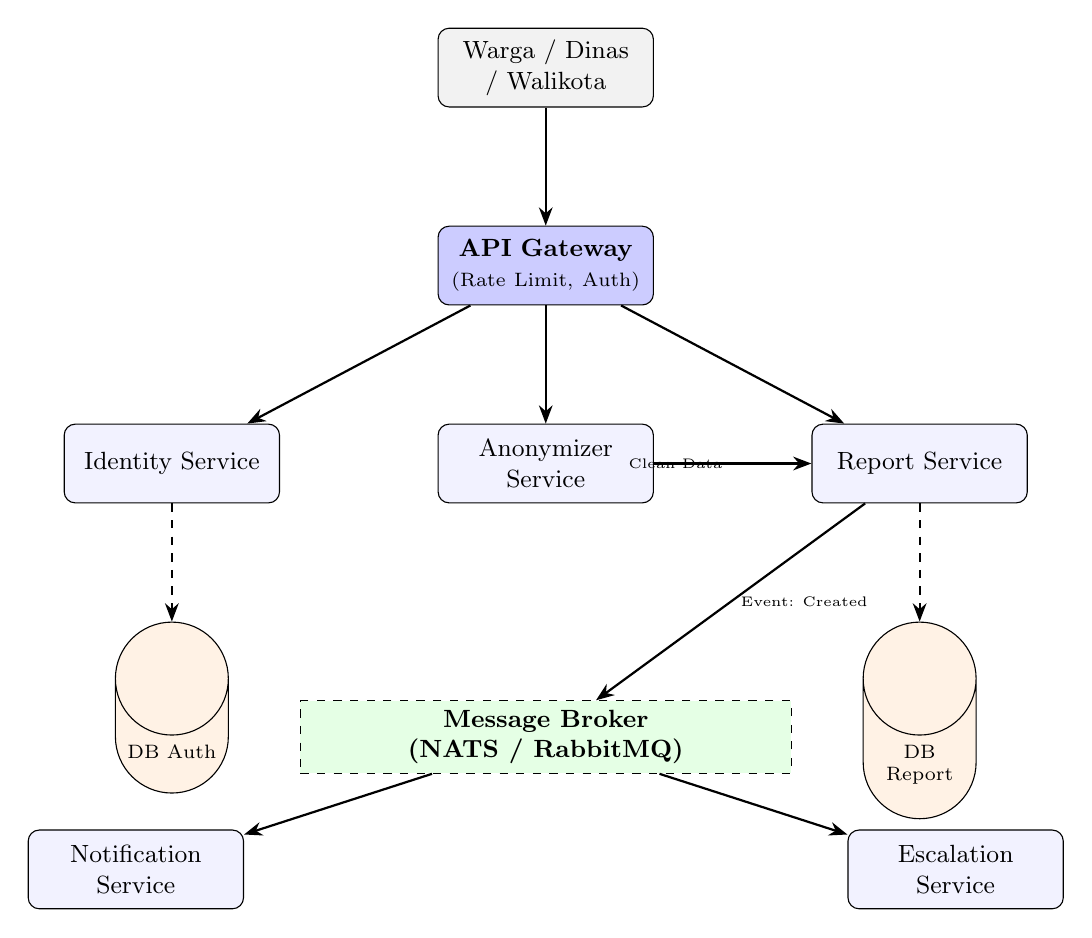
\begin{tikzpicture}[
        node distance=1.5cm and 2cm,
        box/.style={rectangle, draw, fill=blue!5, text width=2.5cm, align=center, minimum height=1cm, rounded corners, font=\small},
        db/.style={cylinder, draw, shape border rotate=90, fill=orange!10, text width=1.2cm, align=center, minimum height=1.5cm, font=\scriptsize},
        broker/.style={rectangle, draw, fill=green!10, text width=6cm, align=center, minimum height=0.8cm, dashed, font=\small\bfseries},
        arrow/.style={-Stealth, thick}
    ]

    % Aktor
    \node (user) [box, fill=gray!10] {Warga / Dinas / Walikota};
    
    % Gateway
    \node (gateway) [box, below=of user, fill=blue!20] {\textbf{API Gateway}\\ \scriptsize (Rate Limit, Auth)};

    % Services
    \node (auth) [box, below left=of gateway] {Identity Service};
    \node (anonymizer) [box, below=of gateway] {Anonymizer Service};
    \node (report) [box, below right=of gateway] {Report Service};
    
    % Databases
    \node (db_auth) [db, below=of auth] {DB Auth};
    \node (db_report) [db, below=of report] {DB Report};

    % Message Broker
    \node (nats) [broker, below=2.5cm of anonymizer] {Message Broker (NATS / RabbitMQ)};

    % Worker Services
    \node (notif) [box, below left=1cm of nats] {Notification Service};
    \node (escalation) [box, below right=1cm of nats] {Escalation Service};

    % Garis Hubung
    \draw [arrow] (user) -- (gateway);
    \draw [arrow] (gateway) -- (auth);
    \draw [arrow] (gateway) -- (anonymizer);
    \draw [arrow] (gateway) -- (report);
    
    \draw [arrow, dashed] (auth) -- (db_auth);
    \draw [arrow, dashed] (report) -- (db_report);
    
    \draw [arrow] (report) -- (nats) node[midway, right, font=\tiny] {Event: Created};
    \draw [arrow] (anonymizer) -- (report) node[midway, left, font=\tiny] {Clean Data};
    
    \draw [arrow] (nats) -- (notif);
    \draw [arrow] (nats) -- (escalation);

    \end{tikzpicture}
    \caption{Diagram Arsitektur Logis JagaWarga}
    \label{fig:arch_logic}
\end{figure}

\begin{enumerate}
    \item \textbf{API Gateway:} Bertindak sebagai titik masuk tunggal. Bertanggung jawab atas \textit{routing}, \textit{authentication check}, dan \textit{rate limiting}.
    \item \textbf{Identity Service:} Menangani pendaftaran dan validasi identitas warga untuk memastikan data pelapor asli (\textbf{NFR-S3}), namun tetap memisahkan kredensial dari data laporan.
    \item \textbf{Report Service:} Mengelola penyimpanan dan pengambilan data laporan (teks, lokasi, multimedia).
    \item \textbf{Anonymization Service:} Komponen krusial yang bertugas memotong relasi antara identitas pengguna dengan laporan jika kategori laporan dipilih sebagai "Anonim" (\textbf{NFR-S4}).
    \item \textbf{Notification Service:} Mengirimkan pembaruan status laporan kepada warga secara \textit{asynchronous}.
    \item \textbf{Escalation Service:} Layanan berbasis \textit{worker} yang memantau batas waktu penyelesaian laporan dan memicu perpindahan wewenang jika terjadi keterlambatan.
\end{enumerate}

\subsection{Pola Komunikasi Antar-Komponen}
Sistem JagaWarga mengadopsi pendekatan \textit{hybrid communication} untuk menyeimbangkan antara kebutuhan \textit{user experience} yang responsif dan ketangguhan sistem secara keseluruhan.

\subsubsection{Komunikasi Sinkron (Synchronous)}
Komunikasi sinkron menggunakan protokol \textbf{REST} atau \textbf{gRPC} diterapkan pada alur kerja yang membutuhkan kepastian respon seketika (\textit{immediate consistency}).
\begin{itemize}
    \item \textbf{Penggunaan:} Interaksi antara \textit{Gateway} ke \textit{Identity Service} untuk autentikasi, serta pengambilan data laporan publik untuk tampilan utama aplikasi.
    \item \textbf{Justifikasi (NFR-P1):} Protokol gRPC dipilih untuk komunikasi antar-layanan internal karena menggunakan \textit{Protocol Buffers} yang memiliki \textit{payload} lebih kecil dan latensi lebih rendah dibandingkan JSON tradisional, mendukung pencapaian target performa pada beban tinggi.
\end{itemize}

\subsubsection{Komunikasi Asinkron (Asynchronous)}
Untuk proses yang bersifat intensif atau melibatkan banyak layanan turunan, digunakan pola \textit{Event-Driven} melalui \textbf{Message Broker}.
\begin{itemize}
    \item \textbf{Mekanisme:} Setelah \textit{Report Service} berhasil menyimpan data ke basis data, layanan tersebut akan mempublikasikan \textit{event} \texttt{ReportCreated} ke \textit{Message Broker}.
    \item \textbf{Justifikasi (NFR-R1 \& NFR-SC1):} 
    \begin{itemize}
        \item \textbf{Decoupling:} \textit{Report Service} tidak perlu mengetahui keberadaan \textit{Notification Service} atau sistem eksternal lainnya. Ini memudahkan penambahan fitur baru di masa depan tanpa mengubah kode layanan inti.
        \item \textbf{Resilience:} Jika terjadi lonjakan laporan warga secara mendadak, \textit{Message Broker} akan bertindak sebagai \textit{buffer}. Layanan pemroses (seperti \textit{Notification}) dapat mengambil pesan sesuai dengan kapasitas kemampuannya (\textit{backpressure handling}), sehingga sistem tidak tumbang akibat \textit{resource exhaustion}.
    \end{itemize}
\end{itemize}

\subsubsection{Analisis Alur Interaksi Pelaporan Anonim}

\begin{figure}[H]
    \centering
    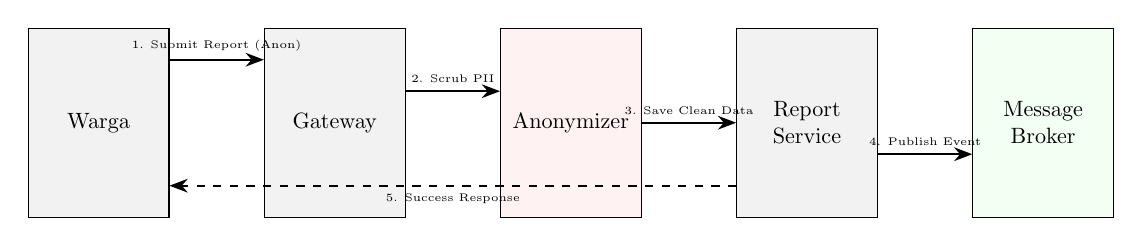
\begin{tikzpicture}[
        scale=0.8, transform shape,
        obj/.style={rectangle, draw, fill=gray!10, text width=2cm, align=center, minimum height=3cm},
        arrow/.style={-Stealth, thick}
    ]

    % Lifelines
    \node (warga) [obj] {Warga};
    \node (gw) [obj, right=1.5cm of warga] {Gateway};
    \node (anon) [obj, right=1.5cm of gw, fill=red!5] {Anonymizer};
    \node (rep) [obj, right=1.5cm of anon] {Report Service};
    \node (nats) [obj, right=1.5cm of rep, fill=green!5] {Message Broker};

    % Alur
    \draw [arrow] ([yshift=1cm]warga.east) -- ([yshift=1cm]gw.west) node[midway, above, font=\tiny] {1. Submit Report (Anon)};
    \draw [arrow] ([yshift=0.5cm]gw.east) -- ([yshift=0.5cm]anon.west) node[midway, above, font=\tiny] {2. Scrub PII};
    \draw [arrow] ([yshift=0cm]anon.east) -- ([yshift=0cm]rep.west) node[midway, above, font=\tiny] {3. Save Clean Data};
    \draw [arrow] ([yshift=-0.5cm]rep.east) -- ([yshift=-0.5cm]nats.west) node[midway, above, font=\tiny] {4. Publish Event};
    
    % Return
    \draw [arrow, dashed] ([yshift=-1cm]rep.west) -- ([yshift=-1cm]warga.east) node[midway, below, font=\tiny] {5. Success Response};

    \end{tikzpicture}
    \caption{Diagram Interaksi Pelaporan Anonim (\textit{Whistleblowing})}
    \label{fig:interaction_anon}
\end{figure}

Berdasarkan \textbf{Gambar \ref{fig:interaction_anon}}, sistem menerapkan prosedur keamanan berlapis untuk menjamin fitur \textit{whistleblowing}:
\begin{enumerate}
    \item \textbf{Submit Report:} Permintaan masuk melalui \textit{Gateway} yang melakukan validasi token JWT pelapor.
    \item \textbf{PII Scrubbing:} Sebelum data menyentuh \textit{persistence layer}, \textit{Anonymizer Service} melakukan transformasi data. Informasi identitas pelapor dipisahkan secara fisik dan hanya ID acak (\textit{pseudonym}) yang diteruskan. Prosedur ini krusial untuk memenuhi \textbf{NFR-S4}.
    \item \textbf{Early Success Response:} Sistem memberikan respon sukses kepada warga segera setelah data tersimpan di \textit{Report Service} (Langkah 5), tanpa menunggu notifikasi terkirim. Hal ini meminimalisir \textit{perceived latency} bagi pengguna.
    \item \textbf{Post-Processing:} Pengiriman notifikasi dan pemicu eskalasi dilakukan sepenuhnya di latar belakang melalui \textit{Message Broker}. Jika \textit{Notification Service} sedang dalam masa \textit{maintenance}, pesan tetap aman tersimpan di antrean (\textit{durability}) dan akan diproses segera setelah layanan kembali aktif.
\end{enumerate}

\section{Pemilihan Teknologi}
Dalam merancang sistem JagaWarga, dipilih pendekatan \textit{Polyglot Architecture} untuk memastikan setiap layanan menggunakan alat yang paling optimal sesuai dengan karakteristik bebannya. Berikut adalah rincian teknologi yang digunakan beserta justifikasinya terhadap kebutuhan fungsional (FR) dan non-fungsional (NFR):

\subsection{Analisis Komponen 1: \textit{Backend Runtime} (Layanan Inti)}
Layanan inti (\textit{core services}) bertanggung jawab atas manajemen laporan, logika eskalasi otomatis, dan integrasi antar-komponen. Mengingat beban target 2,5 juta penduduk, pemilihan \textit{runtime} menjadi krusial untuk menjamin \textit{throughput} tinggi dan \textit{fault tolerance}.

\subsubsection{Alternatif Teknologi yang Memungkinkan}
Dalam tahap perancangan, kami mengevaluasi tiga ekosistem yang memiliki rekam jejak kuat dalam arsitektur terdistribusi:
\begin{enumerate}
    \item \textbf{Node.js (V8 Engine):} Menggunakan model \textit{Event Loop single-threaded} yang sangat efisien untuk operasi I/O intensif namun memiliki batasan pada komputasi paralel murni.
    \item \textbf{Go (Golang):} Bahasa pemrograman yang dikompilasi secara statis dengan fitur \textit{Goroutines}, sangat populer untuk \textit{cloud-native services} karena performa \textit{raw}-nya.
    \item \textbf{Elixir (BEAM VM):} Bahasa fungsional yang berjalan di atas \textit{Erlang Virtual Machine}. Didesain sejak awal untuk sistem terdistribusi (\textit{distributed by nature}) dan \textit{soft real-time}.
\end{enumerate}

\subsubsection{\textit{Pros} dan \textit{Cons} Teknologi}
Berikut adalah tabel perbandingan mendalam berdasarkan kriteria teknis yang relevan dengan aplikasi JagaWarga:

\begin{table}[H]
    \centering
    \small
    \begin{tabular}{@{} p{2.5cm} p{4.5cm} p{4.5cm} @{} }
        \toprule
        \textbf{Teknologi} & \textbf{\textit{Pros}} & \textbf{\textit{Cons}} \\ \midrule
        \textbf{Node.js} & Ekosistem NPM yang masif; \textit{Development velocity} sangat cepat; sangat baik untuk aplikasi \textit{I/O bound}. & \textit{Single-threaded} per \textit{instance}; satu \textit{unhandled exception} dapat mematikan seluruh proses aplikasi. \\ \midrule
        \textbf{Go} & Kompilasi cepat ke \textit{binary} tunggal; konkurensi murah melalui \textit{CSP (Communicating Sequential Processes)}; sangat cepat untuk tugas \textit{CPU-bound}. & Manajemen \textit{error} yang repetitif; tidak memiliki model \textit{fault isolation} bawaan di tingkat \textit{runtime} (bergantung pada orkestrasi luar). \\ \midrule
        \textbf{Elixir} & \textit{Fault tolerance} tingkat tinggi melalui \textit{Supervisor Trees}; \textit{Hot code swapping}; tidak ada \textit{shared state} (menghindari \textit{race conditions}). & Paradigma fungsional memerlukan \textit{learning curve} tambahan; ekosistem \textit{library} lebih spesifik dan tidak sebanyak Node/Go. \\ \bottomrule
    \end{tabular}
    \caption{Perbandingan Mendalam \textit{Backend Runtime}}
\end{table}

\subsubsection{Kesesuaian dengan Aplikasi dan Justifikasi Arsitektural}
Aplikasi JagaWarga memiliki dua tantangan kritis: lonjakan laporan mendadak (NFR-SC1) dan kebutuhan eskalasi otomatis yang tidak boleh berhenti meskipun terjadi error pada salah satu laporan (NFR-R1). 

Kami mengacu pada filosofi \textbf{Joe Armstrong}, salah satu pencipta Erlang, yang menyatakan:
\begin{quote}
    \textit{"If you want to build a system that is reliable, you must build it out of parts that can fail without affecting the whole."}
\end{quote}



Filosofi ini diimplementasikan secara \textit{native} oleh Elixir melalui \textit{Supervisor Trees}. Jika proses eskalasi untuk satu laporan gagal (misalnya karena data korup), proses tersebut akan mati (\textit{crash}) secara terisolasi tanpa mengganggu jutaan proses laporan lainnya, dan akan segera dijalankan ulang (\textit{restart}) oleh \textit{Supervisor}. 

Selain itu, penelitian dari tim \textit{engineering} \textbf{Discord} menunjukkan bahwa Elixir mampu menangani lebih dari 11 juta pengguna \textit{concurrent} dengan model \textit{Actor} yang dimilikinya. Hal ini sangat relevan untuk skenario kota dengan 2,5 juta warga, di mana efisiensi memori per proses jauh lebih penting daripada kecepatan CPU mentah.

\subsubsection{Kesimpulan Teknologi Terpilih}
Berdasarkan analisis di atas, kami memilih \textbf{Elixir (dengan Phoenix Framework)}. Meskipun Go menawarkan eksekusi yang lebih cepat untuk algoritma kompleks, Elixir memberikan \textbf{\textit{Availability}} dan \textbf{\textit{Resilience}} yang tidak tertandingi melalui \textit{BEAM VM}. Keputusan ini secara langsung menjawab tantangan keandalan dan skalabilitas yang menjadi syarat mutlak aplikasi sistem terdistribusi JagaWarga.

\subsection{Analisis Komponen 2: Sistem Basis Data (\textit{Database})}
Sistem basis data merupakan komponen kritikal yang menyimpan seluruh informasi laporan, metadata multimedia, dan data kewenangan instansi. Untuk kota dengan 2,5 juta penduduk, basis data harus mampu menangani volume data yang besar tanpa mengorbankan konsistensi dan ketersediaan (\textit{availability}).

\subsubsection{Alternatif Teknologi yang Memungkinkan}
Terdapat tiga kategori basis data yang dievaluasi untuk kebutuhan arsitektur terdistribusi JagaWarga:
\begin{enumerate}
    \item \textbf{PostgreSQL:} Basis data relasional (RDBMS) tradisional yang sangat matang dan mendukung transaksi ACID secara penuh.
    \item \textbf{MongoDB:} Basis data NoSQL berbasis dokumen yang menawarkan skema fleksibel dan kemudahan dalam melakukan \textit{sharding}.
    \item \textbf{CockroachDB:} Basis data \textit{Distributed SQL} yang dirancang untuk skala \textit{cloud-native} dengan arsitektur \textit{shared-nothing}.
\end{enumerate}

\subsubsection{\textit{Pros} dan \textit{Cons} Teknologi}
Berikut adalah evaluasi mendalam terhadap ketiga kandidat basis data:

\begin{table}[H]
    \centering
    \small
    \begin{tabular}{@{} p{2.5cm} p{4.5cm} p{4.5cm} @{} }
        \toprule
        \textbf{Teknologi} & \textbf{\textit{Pros}} & \textbf{\textit{Cons}} \\ \midrule
        \textbf{PostgreSQL} & Dukungan komunitas dan \textit{tooling} sangat luas; konsistensi data sangat terjamin; performa tinggi pada \textit{single-node}. & Sulit untuk melakukan \textit{horizontal scaling} secara otomatis; risiko \textit{single point of failure} tinggi tanpa manajemen \textit{failover} yang kompleks. \\ \midrule
        \textbf{MongoDB} & Skema JSON-like yang fleksibel; performa tulis yang sangat cepat; \textit{native sharding}. & Konsistensi data sulit dijamin pada transaksi lintas dokumen (\textit{multi-document ACID}) dalam lingkungan terdistribusi. \\ \midrule
        \textbf{CockroachDB} & \textit{Auto-sharding} dan replikasi otomatis; mendukung transaksi ACID penuh dalam skala terdistribusi; \textit{high availability} secara \textit{native}. & Memerlukan sumber daya memori dan CPU yang lebih besar dibandingkan PostgreSQL konvensional; latensi tulis sedikit lebih tinggi karena mekanisme konsensus. \\ \bottomrule
    \end{tabular}
    \caption{Perbandingan Sistem Basis Data}
\end{table}

\subsubsection{Kesesuaian dengan Aplikasi dan Justifikasi Arsitektural}
Tantangan utama sistem JagaWarga adalah \textbf{NFR-SC1} (Skalabilitas) dan \textbf{NFR-R1} (Keandalan). Dalam teori \textbf{CAP Theorem} (Consistency, Availability, Partition Tolerance), sistem terdistribusi biasanya harus mengorbankan salah satu aspek. Namun, CockroachDB yang terinspirasi dari makalah \textbf{Google Spanner} berhasil menyeimbangkan ketiganya melalui protokol konsensus \textbf{Raft}.

Dengan CockroachDB, jika terjadi lonjakan laporan mendadak dari 2,5 juta warga, tim infrastruktur cukup menambah node baru ke dalam klaster, dan basis data akan melakukan \textit{re-balancing} data secara otomatis tanpa \textit{downtime}. Selain itu, mekanisme replikasi 3-node menjamin bahwa jika satu pusat data mengalami kegagalan, sistem tetap dapat melayani permintaan warga tanpa kehilangan data sedikitpun.

\subsubsection{Kesimpulan Teknologi Terpilih}
Dipilih \textbf{CockroachDB} sebagai solusi penyimpanan utama. Meskipun PostgreSQL lebih familiar, kebutuhan akan \textit{horizontal scaling} yang mulus dan jaminan ketersediaan data pada skala kota besar menjadikan CockroachDB sebagai pilihan yang lebih superior untuk memenuhi standar arsitektur terdistribusi yang handal.

\begin{table}[H]
    \centering
    \small
    \begin{tabular}{@{} p{2.5cm} p{2.5cm} p{5.5cm} l @{}}
        \toprule
        \textbf{Komponen} & \textbf{Teknologi} & \textbf{Alasan Pemilihan} & \textbf{Ref. Req} \\ \midrule
        \textbf{Core Service} (Report \& Escalation) & \textbf{Elixir} (Phoenix) & Memanfaatkan BEAM VM untuk \textit{fault tolerance} tinggi melalui \textit{supervisor trees}. Sangat efisien dalam menangani ribuan \textit{process} ringan secara konkuren. & NFR-R1, NFR-SC1, FR-8 \\ \midrule
        \textbf{Identity \& Anonymizer} & \textbf{Bun} (ElysiaJS) & \textit{Runtime} berbasis Zig yang memiliki performa \textit{cold start} dan eksekusi sangat cepat. Mendukung \textit{end-to-end type safety} untuk validasi identitas dan \textit{PII scrubbing}. & NFR-P1, NFR-S2, NFR-S4 \\ \midrule
        \textbf{Message Broker} & \textbf{NATS JetStream} & \textit{Cloud-native messaging system} yang sangat ringan namun mendukung persistensi data dan pola \textit{at-least-once delivery}. & NFR-R1, NFR-SC1, FR-4 \\ \midrule
        \textbf{Main Database} & \textbf{CockroachDB} & \textit{Distributed SQL database} yang mendukung \textit{auto-sharding} dan replikasi data otomatis. Menjamin data tetap tersedia meskipun salah satu node pusat data mati. & NFR-SC1, NFR-S1, NFR-S5 \\ \midrule
        \textbf{API Gateway} & \textbf{Traefik} & \textit{Edge router} yang mendukung konfigurasi dinamis, otomatisasi SSL/TLS, dan integrasi \textit{native} dengan orkestrasi kontainer. & NFR-S5, NFR-SC2 \\ \midrule
        \textbf{Observability} & \textbf{Prometheus \& Grafana} & Standar industri untuk pengumpulan metrik deret waktu (\textit{time-series}) dan visualisasi performa sistem secara \textit{real-time}. & NFR-O1, NFR-O2 \\ \bottomrule
    \end{tabular}
    \caption{Tabel Justifikasi Pemilihan \textit{Tech Stack} JagaWarga}
    \label{tab:tech_stack}
\end{table}



Pemilihan teknologi di atas didasarkan pada prinsip \textit{Survivability} dan \textit{High Scalability}. Penggunaan \textbf{Elixir} dan \textbf{CockroachDB} secara khusus menjawab tantangan pengelolaan 2,5 juta warga, di mana ketersediaan sistem (\textit{availability}) adalah prioritas utama. Sementara itu, penggunaan \textbf{Bun} pada layanan anonimitas memastikan proses transformasi data tidak menjadi hambatan (\textit{bottleneck}) bagi performa keseluruhan aplikasi (\textbf{NFR-P1}).

\section{Perancangan Proof-of-Concept (PoC)}
Mengingat kompleksitas sistem \textit{JagaWarga} secara keseluruhan, dilakukan pembatasan lingkup implementasi pada tahap \textit{Proof-of-Concept} (PoC). Fokus PoC adalah membuktikan bahwa arsitektur terdistribusi yang dirancang mampu menangani alur kerja paling kritis dengan tetap menjaga atribut kualitas yang dipersyaratkan.

\subsection{Fungsionalitas Terpilih}
Fungsionalitas yang dipilih untuk diimplementasikan dalam PoC adalah \textbf{"Alur Pelaporan Anonim dan Mekanisme Eskalasi Otomatis"}. Fitur ini mencakup beberapa kebutuhan fungsional yaitu:
\begin{itemize}
    \item \textbf{FR-1 (Pelaporan Anonim):} Warga mengirim laporan, identitas diproses oleh \textit{Anonymizer}, dan data disimpan tanpa tautan ke identitas asli.
    \item \textbf{FR-5 (Respon Instansi):} Simulasi pihak berwenang menerima dan melihat laporan sesuai kategori.
    \item \textbf{FR-8 (Eskalasi Otomatis):} \textit{Worker} mendeteksi laporan yang melewati batas waktu (\textit{timeout}) dan mengubah statusnya menjadi "Tereskalasi".
\end{itemize}

\subsection{Atribut Kualitas Terpilih}
Atribut kualitas (kebutuhan non-fungsional) yang akan dibuktikan dalam PoC adalah:
\begin{itemize}
    \item \textbf{NFR-R1 (Keandalan/Fault Isolation):} Menunjukkan sistem tetap dapat menerima laporan meskipun salah satu layanan (misal: \textit{Notification Service}) sedang tidak tersedia.
    \item \textbf{NFR-SC1 (Skalabilitas):} Membuktikan penggunaan antrean pesan (\textit{Message Broker}) untuk menangani lonjakan laporan tanpa membebani basis data secara sinkron.
    \item \textbf{NFR-S4 (Proteksi Data Pribadi):} Memastikan \textit{data scrubbing} pada laporan anonim bekerja di tingkat \textit{backend}.
\end{itemize}

\subsection{Alasan Pemilihan}
Pemilihan fitur dan kualitas di atas didasarkan pada argumen berikut:
\begin{enumerate}
    \item \textbf{Representasi Kompleksitas Terdistribusi:} Alur pelaporan anonim hingga eskalasi melibatkan interaksi antar-layanan (Bun, Elixir, dan NATS) serta manipulasi \textit{state} di basis data terdistribusi (CockroachDB). Hal ini merepresentasikan tantangan teknis utama dari sistem.
    \item \textbf{Pembuktian Janji Arsitektur:} Fitur eskalasi otomatis membuktikan kemampuan sistem dalam menjalankan proses latar belakang (\textit{background job}) secara independen, yang merupakan ciri khas arsitektur \textit{microservices}.
    \item \textbf{Mitigasi Risiko Keamanan:} Anonimitas adalah fitur paling krusial dalam aplikasi pelaporan warga (untuk \textit{whistleblowing}). Membuktikan fitur ini di tahap PoC menjamin bahwa fondasi keamanan sistem sudah benar sebelum dikembangkan lebih lanjut.
\end{enumerate}

\section{Detail Implementasi PoC}
Bagian ini menyajikan teknis implementasi dari \textit{Proof-of-Concept} yang telah dirancang untuk membuktikan fungsionalitas dan kualitas sistem terdistribusi \textit{JagaWarga}.

\subsection{Sumber Kode}
Seluruh kode sumber untuk layanan \textit{backend}, konfigurasi infrastruktur, dan \textit{gateway} dapat diakses melalui repositori berikut:
\begin{itemize}
    \item \textbf{Repositori Utama:} \href{https://github.com/anomali-nangor/jagawarga-poc}{https://github.com/anomali-nangor/jagawarga-poc}
\end{itemize}

\subsection{Panduan Menjalankan Sistem}
Sistem telah dikontainerisasi menggunakan Docker untuk memastikan konsistensi lingkungan pengembangan. Berikut adalah langkah-langkah untuk menjalankan PoC:

\begin{lstlisting}[language=bash, caption=Instruksi Menjalankan PoC]
# 1. Clone repositori
git clone https://github.com/anomali-nangor/jagawarga-poc.git
cd jagawarga-poc

# 2. Menjalankan seluruh layanan dan infrastruktur
# Termasuk CockroachDB Cluster, NATS, Bun Services, dan Elixir Services
docker-compose up -d

# 3. Verifikasi status container
docker ps
\end{lstlisting}

\subsection{Dokumentasi Hasil Implementasi}
Berikut adalah bukti visual dari komponen sistem yang telah berjalan:

\begin{figure}[H]
    \centering
    % \includegraphics[width=0.8\textwidth]{dashboard_grafana.png} 
    \small [Placeholder: Screenshot Dashboard Grafana menunjukkan metrik sistem]
    \caption{Visualisasi Monitoring Sistem melalui Grafana}
    \label{fig:poc_grafana}
\end{figure}

\begin{figure}[H]
    \centering
    % \includegraphics[width=0.8\textwidth]{nats_logs.png}
    \small [Placeholder: Screenshot Log NATS JetStream saat terjadi Event Pelaporan]
    \caption{Log Aliran Pesan Asinkron pada Message Broker}
    \label{fig:poc_nats}
\end{figure}

\section{Asumsi-Asumsi Perancangan}
Dalam menyusun rancangan arsitektur dan implementasi PoC ini, diambil beberapa asumsi sebagai batasan ruang lingkup:
\begin{enumerate}
    \item \textbf{Validitas Identitas:} Sistem mengasumsikan bahwa data kependudukan (NIK/KTP) yang dikirimkan warga sudah divalidasi oleh layanan pihak ketiga eksternal yang terpercaya. PoC hanya fokus pada cara sistem menangani data tersebut setelah divalidasi.
    \item \textbf{Penyimpanan Multimedia:} Dokumen multimedia (foto/video) dalam PoC diasumsikan disimpan dalam \textit{local volume} yang terikat pada kontainer \textit{Report Service}, bukan pada \textit{Object Storage} (seperti S3) yang terdistribusi secara geografis.
    \item \textbf{Waktu Eskalasi:} Untuk kebutuhan demonstrasi, waktu tunggu eskalasi otomatis (FR-8) dipercepat dari satuan hari menjadi satuan detik/menit agar perubahan status dapat terlihat secara \textit{real-time}.
    \item \textbf{Integrasi Eksternal:} Sistem eksternal yang disebutkan pada FR-7 disimulasikan sebagai sebuah \textit{mock webhook} yang mencatat penerimaan data laporan tanpa melakukan pemrosesan lebih lanjut.
    \item \textbf{Keamanan Jaringan:} Seluruh komunikasi antar-layanan di dalam \textit{private network} Docker diasumsikan aman, namun komunikasi publik melalui \textit{Gateway} tetap diwajibkan menggunakan protokol HTTPS/TLS.
\end{enumerate}

\end{document}